\section{Notation and Preliminaries} 
\label{sec:preliminaries}


\begin{wrapfigure}{r}{0.27\textwidth}
\centering
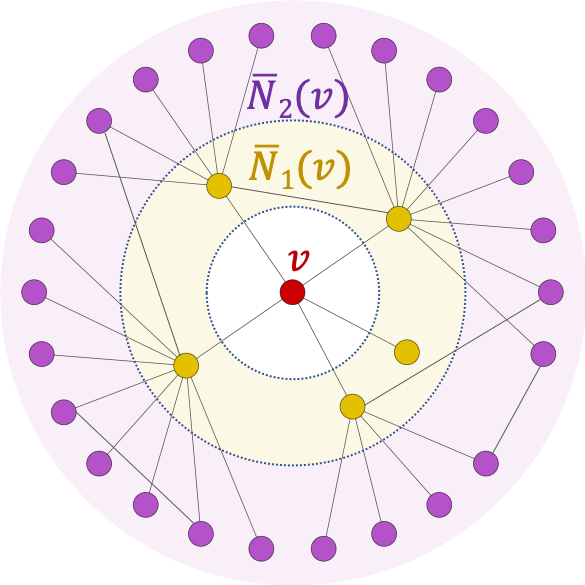
\includegraphics[width=0.25\textwidth]{submissions/Jiong2023/FIG/neighborhoods.png}
\caption{Neighborhoods.}
\label{fig:neighborhoods}
\end{wrapfigure}
In this section, we give the key notations and definitions that we use throughout our paper. 
Let $\graph=(\vertexSet,\edgeSet)$ be an undirected, unweighted graph with node set $\vertexSet$ and edge set $\edgeSet$. 
We denote a general neighborhood centered around $v$ as $N(v)$ ($\graph$ may have self-loops), the corresponding neighborhood that does \textit{not} include the ego (node $v$) as $\neighNoSelfLoop(v)$, and the general neighbors of node $v$ at exactly $i$ hops/steps away (minimum distance) as $\bar{N}_i(v)$. For example, as shown in Fig.~\ref{fig:neighborhoods}, $\bar{N}_1(v) = \{u: (u,v) \in \edgeSet \}$ are the immediate neighbors of $v$.
We represent the graph by 
its adjacency matrix $\matA \in \{0,1\}^{n\times n}$ 
and its node feature matrix $\matX \in \mathbb{R}^{n \times F}$, where 
the vector $\jV{x}_v$ corresponds to the \textit{ego-feature} of node $v$, 
and $\{\jV{x}_u: u \in \neighNoSelfLoop(v)\}$ to its \textit{neighbor-features}. 
We further represent the degree of a node $v$ by $d_v$, which denotes the number of neighbors in its immediate neighborhood $\bar{N}_1(v)$.

We further assume a class label vector $\vecy$, which for each node $v$ contains a unique class label $y_v \in \setY$, and the one-hot encoding $\mathrm{onehot}(y_v)$ forms the row vectors of label encoding matrix $\mathbf{Y} \in \{0,1\}^{n \times |\setY|}$. We further define $\vertexSet_i$ as the set of nodes $v \in \vertexSet$ with label $y_v = i$.
The goal of semi-supervised node classification is to learn a mapping $\ell: \vertexSet \rightarrow \setY$, given a set of labeled nodes $\setT = \{(v_1,y_1), (v_2, y_2), ...\}$ as training data.  


\paragraph{Graph Neural Networks (GNNs).} 
\label{sec:2-gnn}
From a probabilistic perspective, most GNN models assume the following local Markov property on node features: 
for each node $v \in \vertexSet$, there exists a neighborhood $N(v)$ such that
$y_v$ only depends on the ego-feature $\jV{x}_v$ and neighbor-features $\{\jV{x}_u: u \in N(v)\}$. 
Most models derive the class label $y_v$ via the following representation learning approach: {\small 
\begin{equation}
    \jV{r}^{(k)}_v = f\left(\jV{r}^{(k-1)}_v, \{\jV{r}^{(k-1)}_u: u \in N(v)\}\right),     \; \jV{r}^{(0)}_v = \jV{x}_v, \; \text{and} \;  y_v = \arg \max \{\mathrm{softmax}(\jV{r}^{(K)}_v)\matW\},
    \label{eq:gnn}
\end{equation}
}
where the embedding function $f$ is applied repeatedly in $K$ total rounds, 
node $v$'s representation (or hidden state vector) at round $k$, {\small $\jV{r}^{(k)}_v$}, is learned from its ego- and neighbor-representations in the previous round, and a softmax classifier with {learnable weight matrix} $\matW$ is applied to the final representation of $v$.
Most existing models differ in their definitions of neighborhoods $N(v)$ and embedding function $f$. 
A typical definition of neighborhood is $N_1(v)$---i.e., the 1-hop neighbors of $v$. 
As for $f$, in graph convolutional networks (GCN)~\cite{kipf2016semi} each node repeatedly averages its own features and those of its neighbors to update its own feature representation.  Using an attention mechanism, GAT~\cite{velickovic2018graph} models the influence of different neighbors more precisely as a weighted average of the ego- and neighbor-features. GraphSAGE~\cite{hamilton2017inductive} generalizes the aggregation beyond averaging, and models the ego-features distinctly from the neighbor-features in its subsampled neighborhood.


\paragraph{Homophily and heterophily.} 
\label{sec:homophily}

\begin{wrapfigure}{r}{0.33\textwidth}
    \vspace{-0.4cm}
    \centering
    \adjincludegraphics[width=0.3\textwidth, trim={0 0 0 {0.13\height}}, clip]{submissions/Jiong2023/FIG/example-graph.pdf}
    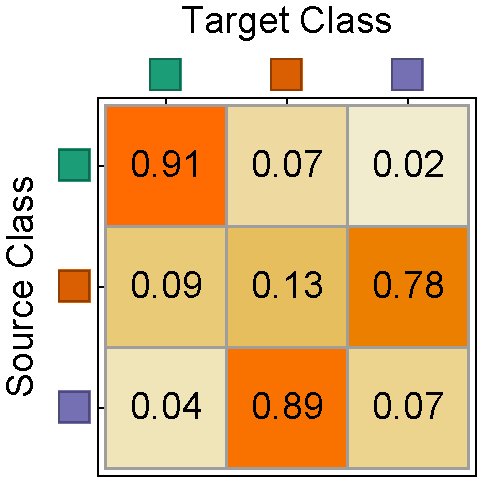
\includegraphics[width=0.2\textwidth]{submissions/Jiong2023/FIG/example-graph-comp.pdf}
    \caption{An example graph (top) and its empirical class compatibility matrix $\matH$ (bottom). It demonstrates mixed \emph{homophily} and \emph{heterophily}, with node colors represent class labels: nodes in green show strong homophily, while nodes in orange and purple show strong heterophily.}
    \label{fig:mixed-heterophily-example}
    \vspace{-0.9cm}
\end{wrapfigure}
In this work, we focus on heterophily in class labels. We first define the edge homophily ratio $h$ as a measure of the graph homophily level, and use it to define graphs with strong homophily/heterophily: 
\begin{definition}[Edge Homophily Ratio~\cite{MixHop,zhu2020beyond}]
The edge homophily ratio $h = \tfrac{|\{(u,v): (u,v) \in \edgeSet \wedge y_u = y_v\}|}{|\edgeSet|}$ is the fraction of edges in a graph which connect nodes that have the same class label (i.e., intra-class edges). 
\label{dfn:homophily-ratio}
\end{definition}
\begin{definition}\label{dfn:heterophily-nets}
Graphs with strong homophily have high edge homophily ratio $h  \rightarrow 1$, while graphs with strong heterophily (i.e., low/weak homophily) have small edge homophily ratio $h \rightarrow 0$. 
\end{definition}

The edge homophily ratio in Dfn.~\ref{dfn:homophily-ratio} gives an \textit{overall trend} for all the edges in the graph. The actual level of homophily may vary within different pairs of node classes, i.e., there is different tendency of connection between each pair of classes. 
For instance, in an online purchasing network~\cite{netprobe07} with three classes---fraudsters, accomplices, and honest users---, fraudsters connect with higher probability to accomplices and honest users. 
Moreover, within the same network, it is possible that some classes exhibit homophily, while others exhibit heterophily; we give an example in Figure~\ref{fig:mixed-heterophily-example}.
To capture the tendency of connection between each pair of classes, we define the empirical \textit{class compatibility matrix} $\matH$ as follows: %

\begin{definition}[Empirical Class Compatibility Matrix~\cite{zhu2020beyond,zhu2021graph}]
\label{dfn:compatibility-matrix-empirical}
The empirical class compatibility matrix $\matH$ has entries $[\matH]_{i,j}$ that capture the fraction of edges from a node in class $i$ to a node in class $j$: 
\begin{equation*}
    [\matH]_{i,j} = \frac{|\{(u,v): (u,v) \in \edgeSet \wedge y_u = i \wedge y_v = j\}|}{|\{(u,v): (u,v) \in \edgeSet \wedge y_u = i\}|}
\end{equation*}
\end{definition}
By definition, the class compatibility matrix is a stochastic matrix, with each row summing up to 1. 


\paragraph{Heterophily $\neq$ Heterogeneity.} 
We remark that heterophily, which we study in this work, is a distinct network concept from heterogeneity. 
Formally, a network is heterogeneous~\cite{SunH12} if it has at least two types of nodes and different relationships between them, and homogeneous if it has a single type of nodes (e.g., users) and a single type of edges (e.g., friendship). The type of nodes in heterogeneous graphs does \textit{not} necessarily match the class labels $y_v$, therefore both homogeneous and heterogeneous networks may have different levels of homophily. 













